\documentclass{article}

\usepackage{graphicx}
\usepackage{tikz}
\usepackage{tikzsymbols}
\usetikzlibrary{calc,patterns,shapes.geometric}
\pagestyle{empty}
\usepackage[margin=0pt]{geometry}
\geometry{papersize={14in,12in}}

\def\centerarc[#1](#2)(#3:#4:#5){\draw[#1] ($(#2)+({#5*cos(#3)},{#5*sin(#3)})$) arc (#3:#4:#5);}

\begin{document}
	\begin{figure}
		\centering
		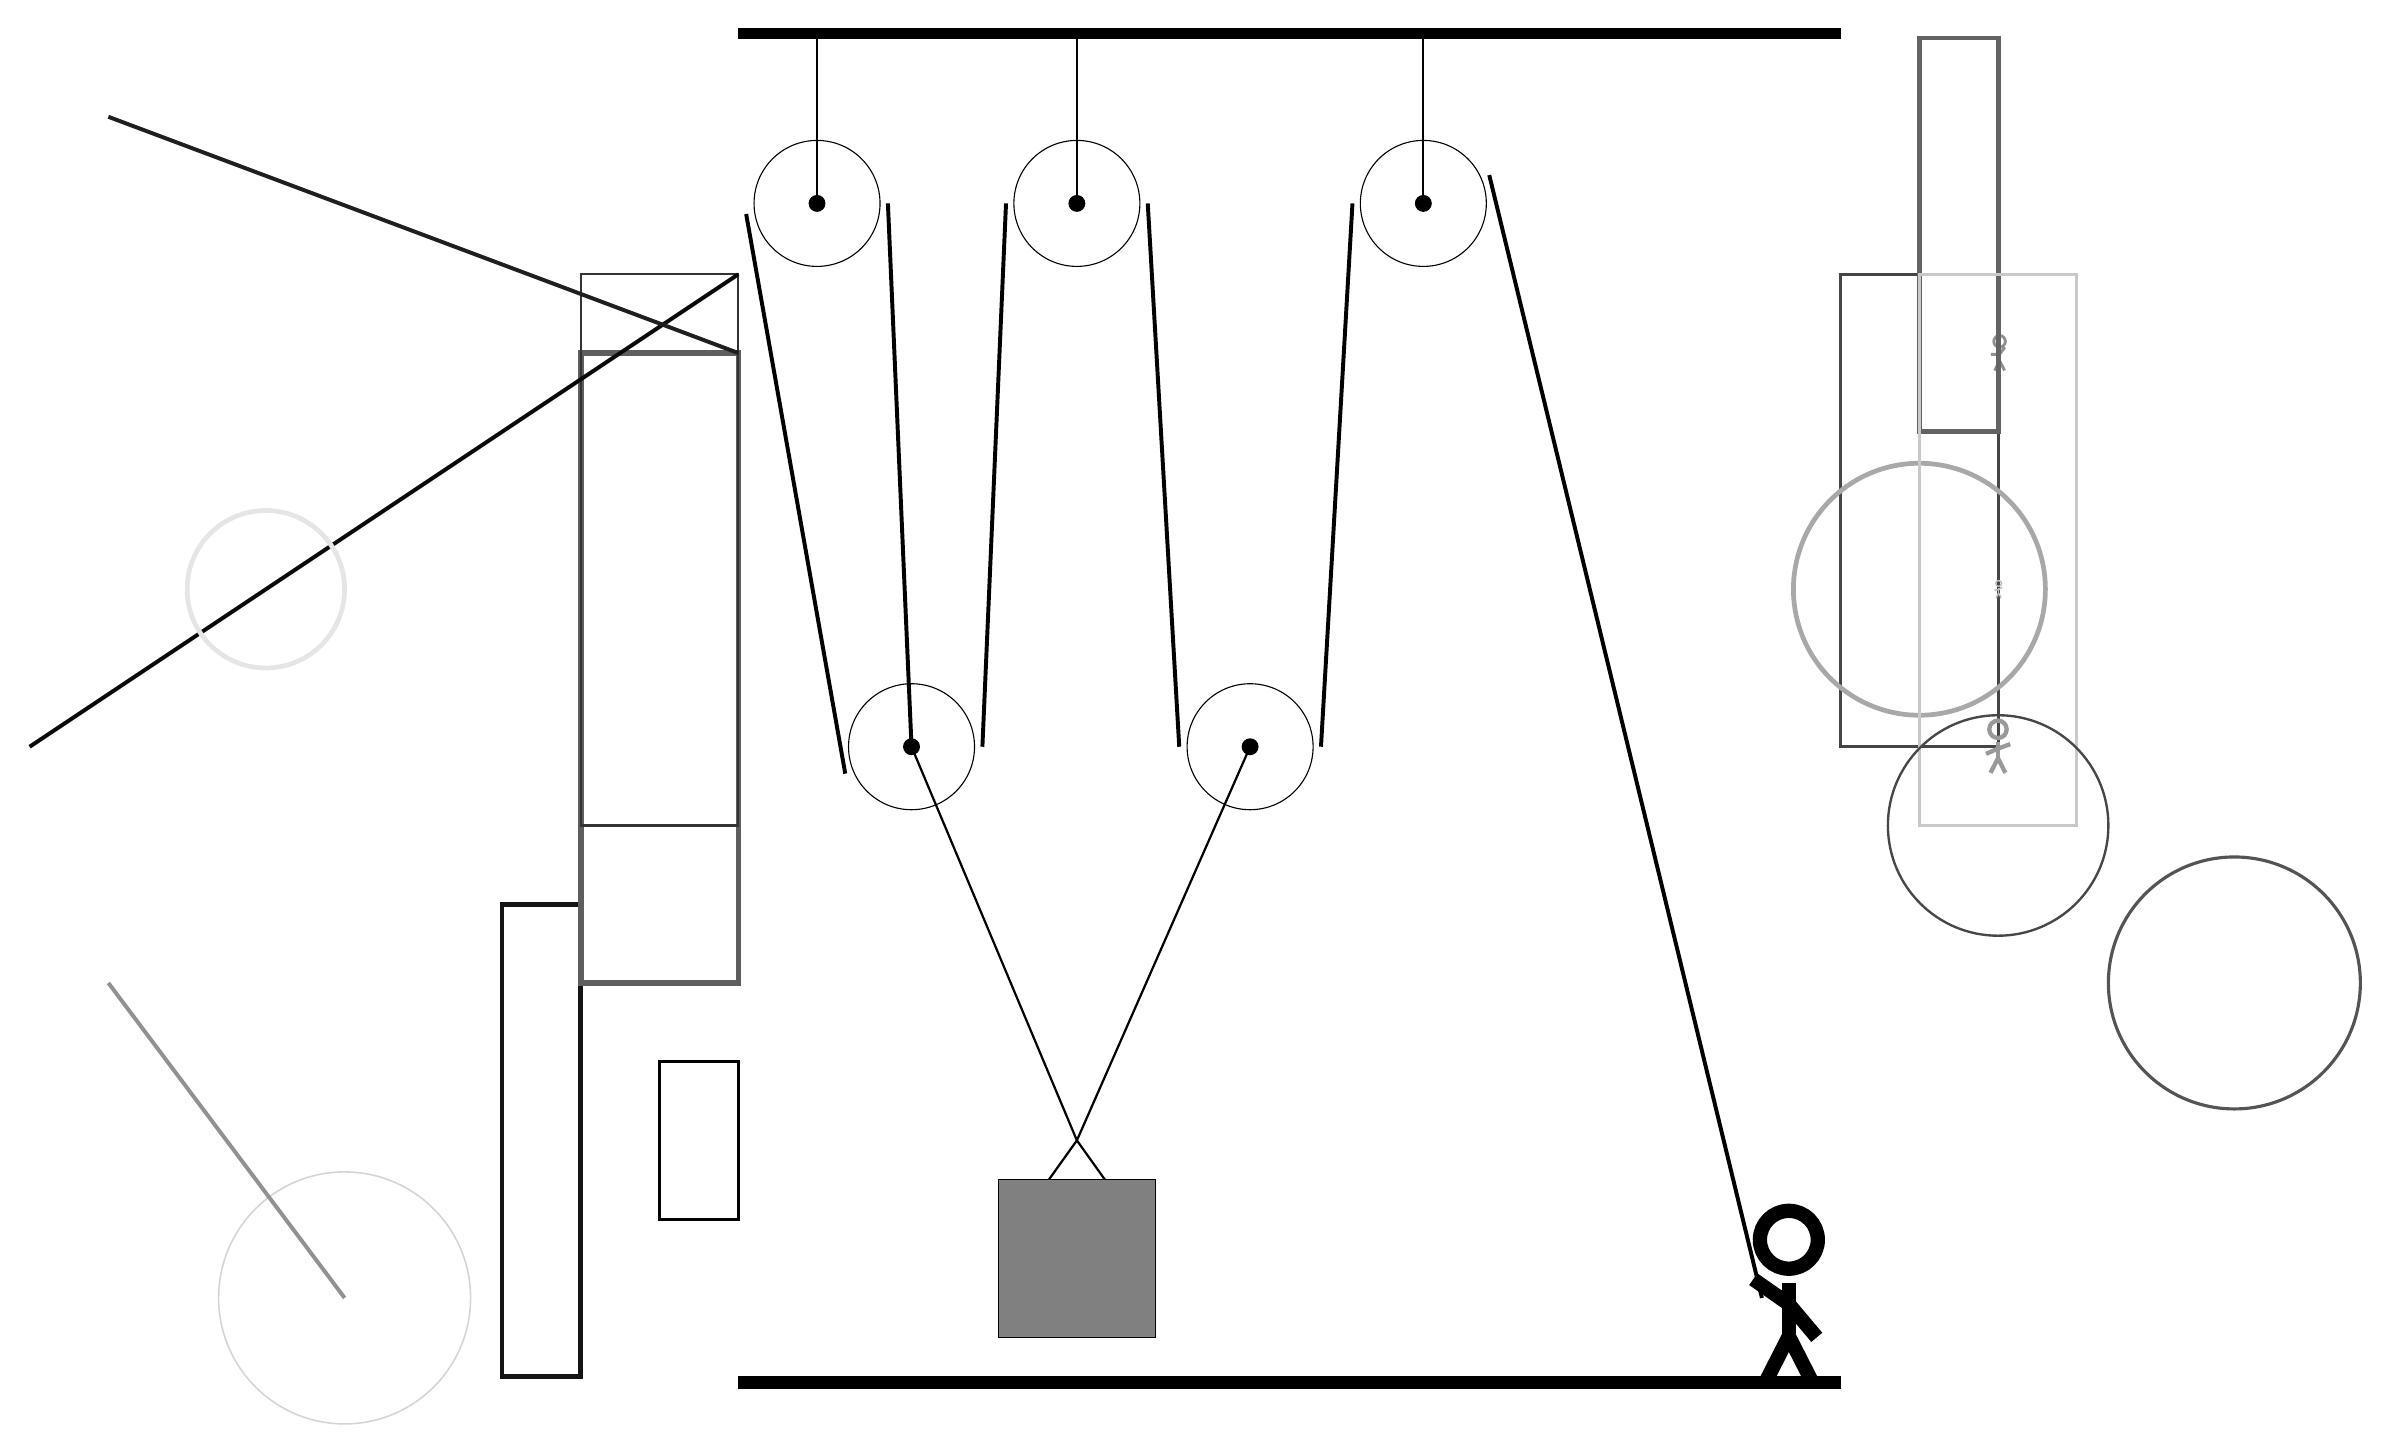
\begin{tikzpicture}
			%%%%% START %%%%%
			
			\draw[fill=black] (-2, 14) rectangle (12, 14.125);
			
			\draw (-1, 11.9) circle (0.8);
			\draw[fill=black] (-1, 11.9) circle (0.1);
			\draw[thick] (-1, 11.9) -- (-1, 14);
			
			\draw[line width=0.4mm, color=black!73] (14, 11) rectangle (12, 5);
			
			\node[line width=0.2mm, color=black!44] at (14, 10) {\Strichmaxerl[2][1][53]};
			\draw[line width=0.4mm, color=black!100] (-3, 1) rectangle (-2, -1);
			\draw[line width=0.6mm, color=black!61] (13, 9) rectangle (14, 14);
			\draw [line width=0.4mm, color=black!67](17, 2) circle (1.6);
			
			\draw [line width=0.6mm, color=black!34](13, 7) circle (1.6);
			\draw[line width=0.6mm, color=black!92] (-4, 3) rectangle (-5, -3);
			\draw[line width=0.7mm, color=black!63] (-2, 10) rectangle (-4, 2);
			\node[line width=0.2mm, color=black!40] at (14, 5) {\Strichmaxerl[3][24][20]};
			
			\draw[line width=0.4mm, color=black!21] (13, 11) rectangle (15, 4);
			
			\draw[line width=0.3mm, color=black!80] (-4, 4) rectangle (-2, 11);
			\node[line width=0.2mm, color=black!26] at (14, 7) {\Strichmaxerl[1][3][39]};
			\draw [line width=0.2mm, color=black!17](-7, -2) circle (1.6);
			
			\draw[line width=0.5mm, color=black!43](-7, -2) -- (-10, 2);
			\draw[line width=0.5mm, color=black!96](-2, 11) -- (-11, 5);
			\draw [line width=0.3mm, color=black!72](14, 4) circle (1.4);
			
			\draw [line width=0.6mm, color=black!10](-8, 7) circle (1.0);
			\draw[line width=0.5mm, color=black!88](-2, 10) -- (-10, 13);
			
			\draw (2.3, 11.9) circle (0.8);
			\draw[fill=black] (2.3, 11.9) circle (0.1);
			\draw[thick] (2.3, 11.9) -- (2.3, 14);
			
			\draw (6.7, 11.9) circle (0.8);
			\draw[fill=black] (6.7, 11.9) circle (0.1);
			\draw[thick] (6.7, 11.9) -- (6.7, 14);
			
			\draw (0.2, 5) circle (0.8);
			\draw[fill=black] (0.2, 5) circle (0.1);
			
			\draw (4.5, 5) circle (0.8);
			\draw[fill=black] (4.5, 5) circle (0.1);
			
			\draw[thick] (0.2, 5) -- (2.3, 0)  -- (4.5, 5);
			\draw[thick]  (1.8, -0.7) -- (2.3, 0) -- (2.8, -0.7);
			\draw[fill=black!50] (1.3, -0.5) rectangle (3.3, -2.5);
			
			\draw[line width=0.5mm] (0.2, 5) -- (-0.1, 11.9);
			\centerarc[line width=0.5mm](-1, 11.9)(0:200:0.9);
			\draw[line width=0.5mm] (-1.9, 11.765) -- (-0.6415, 4.658);
			\centerarc[line width=0.5mm](0.2, 5)(200:360:0.9);
			\draw[line width=0.5mm](1.1, 5) -- (1.4, 11.9);
			\centerarc[line width=0.5mm](2.3, 11.9)(0:180:0.9);
			\draw[line width=0.5mm] (3.2, 11.9) -- (3.6, 5);
			\centerarc[line width=0.5mm](4.5, 5)(180:360:0.9);
			\draw[line width=0.5mm] (5.4, 5) -- (5.8, 11.9);
			\centerarc[line width=0.5mm](6.7, 11.9)(20:180:0.9);
			\draw[line width=0.5mm](7.537, 12.26)  -- (11, -2);
			
			\node at (11.3, -2) {\Strichmaxerl[10][-35][-50]};
			
			\draw[fill=black] (-2, -3) rectangle (12, -3.15);
			
			%%%%% END %%%%%
		\end{tikzpicture}
	\end{figure}	
\end{document}